\documentclass[xcolor=svgnames]{beamer}
\usetheme{Warsaw}
\usecolortheme{seahorse}
\usepackage[T1]{fontenc}
\usepackage{graphicx}
\newtheorem{thm}{Theorem}[section]
\newtheorem{claim}[thm]{Claim}
\newtheorem{conj}[thm]{Conjecture}
\newtheorem{cor}[thm]{Corollary}
\newtheorem{conclusion}{Conclusion}
\newtheorem{qu}[thm]{Question}
\newtheorem{remark}[thm]{Remark}
\newtheorem{prop}[thm]{Proposition}
\newtheorem{prob}[thm]{Problem}
\newtheorem{exam}[thm]{Example}
\newtheorem{defn}[thm]{Definition}
\setbeamercovered{transparent}
\setbeamertemplate{navigation symbols}{} % remove navigation symbols

% The original template source code modified to include slide numbers
\setbeamertemplate{footline}{%
  \leavevmode%
  \hbox{\begin{beamercolorbox}[wd=.5\paperwidth,ht=2.5ex,dp=1.125ex,leftskip=.3cm plus1fill,rightskip=.3cm]{author in head/foot}%
    \usebeamerfont{author in head/foot}\insertshortauthor
  \end{beamercolorbox}%
  \begin{beamercolorbox}[wd=.5\paperwidth,ht=2.5ex,dp=1.125ex,leftskip=.3cm,rightskip=.3cm plus1fil]{title in head/foot}%
    \usebeamerfont{title in head/foot}\insertshorttitle\nobreak\hfill\insertframenumber/\inserttotalframenumber
  \end{beamercolorbox}}%
  \vskip0pt%
}

\definecolor{Champagne}{rgb}{0.992, 0.922, 0.75}
\definecolor{LightPink}{rgb}{0.95, 0.85, 0.9}
\definecolor{BlueGray}{rgb}{0.332, 0.406, 0.563}
\definecolor{DeepBlue}{rgb}{0.0, 0.2, 0.4}
\definecolor{DeepPlum}{rgb}{0.45, 0.2, 0.65}
\definecolor{VibrantPurple}{rgb}{0.45, 0.15, 0.75}

\setbeamercolor{palette primary}{bg=LightPink,fg=DeepBlue}
\setbeamercolor{palette secondary}{bg=Champagne,fg=DeepBlue}
\setbeamercolor{palette tertiary}{bg=BlueGray,fg=white}

\setbeamercolor{title}{bg=LightPink,fg=VibrantPurple}
\setbeamercolor{frametitle}{fg=DeepPlum,bg=LightPink}
\setbeamerfont{title}{series=\bfseries}
\setbeamerfont{frametitle}{series=\bfseries}

\setbeamercolor{block title}{fg=Champagne}
\setbeamercolor{block title example}{fg=Champagne}

\renewcommand{\emph}[1]{\textcolor{VibrantPurple}{\textbf{#1}}}

\usepackage{amsmath,amsxtra,amssymb,amsthm,amsfonts}
\usepackage{mathtools}
\usepackage{bm}
\usepackage{unicode-math}
\usepackage{tikz}
\setbeamertemplate{caption}[numbered]

% nice-looking footnotes in slides
\usepackage[absolute,overlay]{textpos}
\newenvironment{reference}[2]{%
  \begin{textblock*}{\textwidth}(#1,#2)
  \footnotesize\it\bgroup\color{DeepBlue}}{\egroup
\end{textblock*}}


\newcommand{\bra}[1]{\langle #1 |}
\newcommand{\ket}[1]{| #1 \rangle}
\newcommand{\braket}[2]{\langle #1 | #2 \rangle}
\newcommand{\ketbra}[2]{| #1 \rangle\langle #2 |}
\newcommand{\bb}[1]{\mathbb{#1}}
\newcommand{\cl}[1]{\mathcal{#1}}
\newcommand\iprod[2]{\ensuremath{\langle#1|#2\rangle}}
\newcommand\oprod[2]{\ensuremath{|#1\rangle\langle#2|}}
\newcommand\ip[2]{\ensuremath{\langle#1 , #2\rangle}}
\newcommand\ave[1]{\ensuremath{\langle #1\rangle}}
\newcommand\Tr{\mathop{\rm Tr}\nolimits}
\newcommand\tr{\mathop{\rm tr}\nolimits}
\newcommand\supp{\mathop{\rm supp}\nolimits}
\newcommand\range{\mathop{\rm range}\nolimits}
\newcommand\argmax{\mathop{\rm argmax}\nolimits}
\newcommand\trho{\tilde{\rho}}
\newcommand\tsigma{\tilde{\sigma}}
\newcommand{\norm}[1]{\|#1\|}
\newcommand{\abs}[1]{\left\lvert #1 \right\rvert}
\newcommand{\floor}[1]{\left\lfloor #1 \right\rfloor}
\newcommand{\ceil}[1]{\left\lceil #1 \right\rceil}
\newcommand{\Innerproduct}[1]{\langle{#1}\rangle}
\newcommand{\afunc}[1]{\operatorname{\mathsf{#1}}}
\newcommand{\defeq}{\stackrel{\smash{\textnormal{\tiny def}}}{=}}

\newcommand{\bij}{%
  \hookrightarrow\mathrel{\mspace{-15mu}}\rightarrow
}

\makeatletter
\newcommand{\xbij}[2][]{%
  \lhook\joinrel
  \ext@arrow 0359\rightarrowfill@ {#1}{#2}%
  \mathrel{\mspace{-15mu}}\rightarrow
}
\makeatother

\usepackage{algorithm,algpseudocode}
\algnewcommand\algorithmicforeach{\textbf{for each}}
\algdef{S}[FOR]{ForEach}[1]{\algorithmicforeach\ #1\ \algorithmicdo}

\algnewcommand{\algorithmicand}{\textbf{ and }}
\algnewcommand{\algorithmicor}{\textbf{ or }}
\algnewcommand{\algorithmicnot}{\textbf{ not }}
\algnewcommand{\algorithmicbreak}{\textbf{break}}
\algnewcommand{\algorithmiccontinue}{\textbf{continue}}
\algnewcommand{\AND}{\algorithmicand}
\algnewcommand{\OR}{\algorithmicor}
\algnewcommand{\NOT}{\algorithmicnot}
\algnewcommand{\BREAK}{\algorithmicbreak}
\algnewcommand{\CONTINUE}{\algorithmiccontinue}

\algrenewcommand\algorithmiccomment[1]{\hfill{\color{gray}\(\triangleright\)
#1}}

\makeatletter
\newcommand{\LeftComment}[1]{%
  \Statex
  {%
    \setlength\leftskip{\ALG@thistlm}%
    \noindent
    \color{gray}\(\triangleright\)\enspace#1\par%
  }%
}

\newcommand{\LeftCommentIndent}[1]{%
  \Statex
  {%
    \setlength\leftskip{\dimexpr\ALG@thistlm+\algorithmicindent}%
    \noindent
    \color{gray}\(\triangleright\)\enspace#1\par%
  }%
}
\makeatother

\def\I{\mathbb{1}}
\def\O{\mathbb{O}}
\def\C{\mathbb{C}}
\def\N{\mathbb{N}}
\def\Z{\mathbb{Z}}
\def\Q{\mathbb{Q}}
\def\R{\mathbb{R}}
\def\E{\mathbb{E}}
\def\F{\mathbb{F}}

\def\B{\mathcal{B}}
\def\D{\mathcal{D}}
\def\Ein{\mathcal{E}}
\def\K{\mathcal{K}}
\def\Lin{\mathcal{L}}
\def\M{\mathcal{M}}
\def\S{\mathcal{S}}
\def\U{\mathcal{U}}
\def\V{\mathcal{V}}
\def\W{\mathcal{W}}
\def\X{\mathcal{X}}
\def\Y{\mathcal{Y}}

\def\a{\mathbf{a}}
\def\b{\mathbf{b}}
\def\c{\mathbf{c}}
\def\d{\mathbf{d}}
\def\e{\mathbf{e}}
\def\p{\mathbf{p}}
\def\q{\mathbf{q}}
\def\r{\mathbf{r}}
\def\u{\mathbf{u}}
\def\vv{\mathbf{v}} % To avoid overriding `\v` (caron diacritic)
\def\w{\mathbf{w}}
\def\x{\mathbf{x}}
\def\y{\mathbf{y}}
\def\z{\mathbf{z}}
\def\0{\mathbf{0}}
\def\1{\mathbf{1}}

\newcommand{\lvnote}[1]{\textcolor{teal}{\textbf{LV:} #1}}

\title[$k$-Incoherent Decomposition Heuristics]{
    Spectral Heuristics for $k$-Incoherent Decompositions
}
\author[L. M. B. Varona]{
    \\[-0.5em]
    \hspace*{-0.75ex}
\includegraphics[width=3cm]{assets/mta_logo.png} \\[0.5em]
    Luis M. B. Varona\inst{1,2,3}
}
\institute[Mount Allison University]{
    Atlantic Undergraduate Physics and Astronomy Conference 2026 \\
    University of Prince Edward Island, Charlottetown, PE
}
\date[March 7, 2026]{March 7, 2026}

\begin{document}

\begin{frame}
    \vspace*{-0.5cm}
    \titlepage
    \begin{reference}{10mm}{83mm}
        \rule{4cm}{0.5pt} \\
        \tiny
        \textsuperscript{1}Department of Politics \& International Relations, Mount Allison University \\
        \textsuperscript{2}Department of Economics, Mount Allison University \\
        \textsuperscript{3}Department of Mathematics \& Computer Science, Mount Allison University \par
    \end{reference}
\end{frame}

\section{Background and Preliminaries}

\subsection{Basic Background}

\frame{
    \frametitle{Quantum Computing and Information}
    \begin{itemize}
        \item Quantum computers use \emph{qubits}, not classical \emph{bits} ($0$ or $1$)
        \uncover<2->{%
        \item A qubit $\ket{\psi} = \alpha\ket{0} + \beta\ket{1}$ is a \emph{superposition} of ``$0$'' and ``$1$,'' where $\alpha, \beta \in \C$ are probability amplitudes with $\lvert\alpha\rvert^2 + \lvert\beta\rvert^2 = 1$ 
        }%
        \uncover<3->{%
            \item Quantum computers can solve (certain) problems far faster, but are highly susceptible to \emph{decoherence}
        }%
        \uncover<4->{%
            \item Recall the thought experiment of \emph{Schr\"{o}dinger's cat(s)}:
        }%
    \end{itemize}
    \begin{figure}
        \centering
        \vspace*{-0.05cm}
        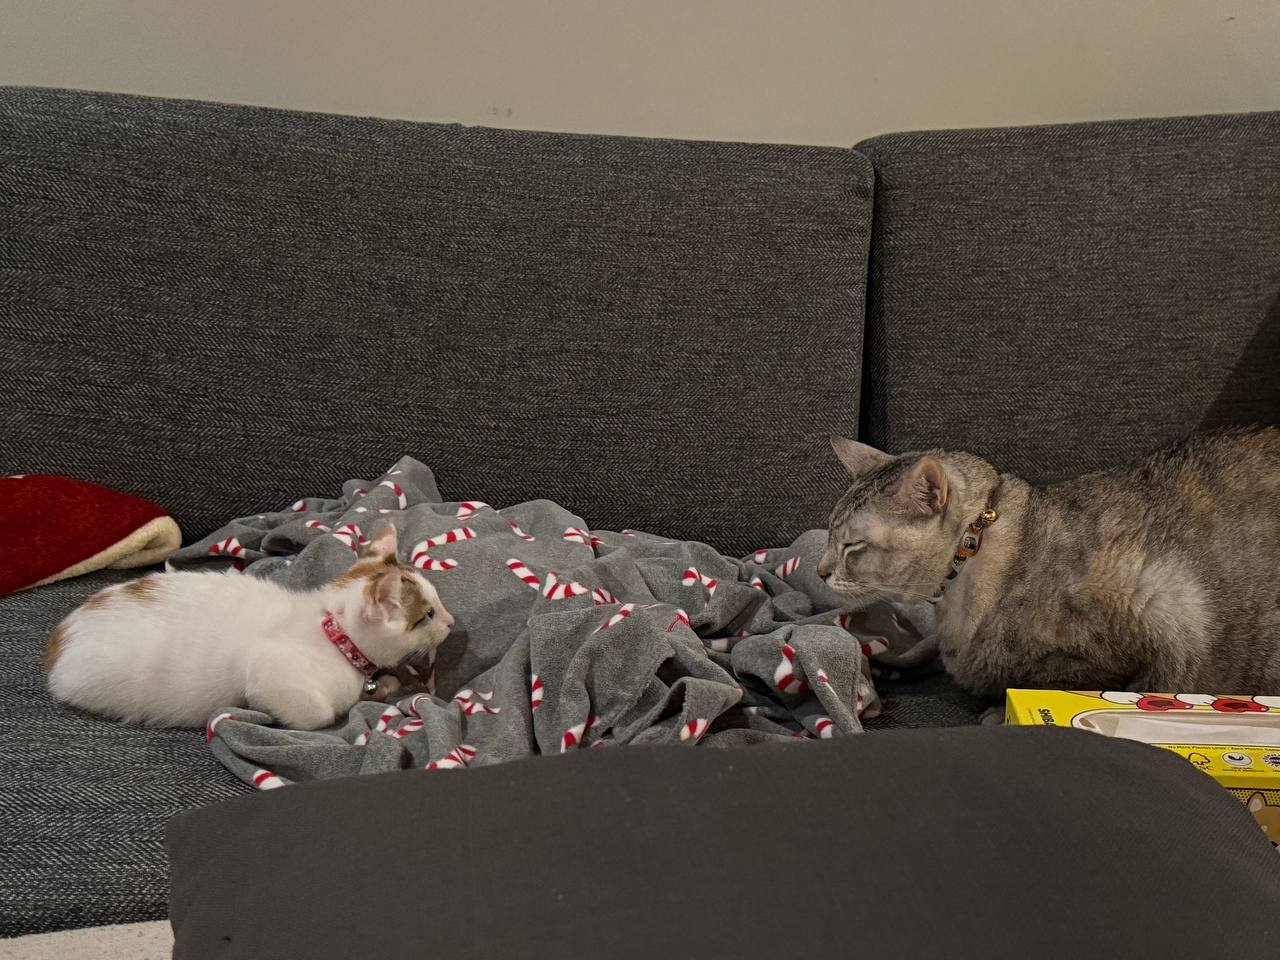
\includegraphics[height=4cm]{assets/yuki_and_ash.JPG}
        \vspace*{-0.3cm}
        \uncover<4->{%
            \caption{My cats, \emph{Yuki} (left) and \emph{Ash}, may be both \emph{awake} and \emph{asleep}~\ldots}
            \label{fig:yuki-and-ash}
        }%
    \end{figure}
}

\subsection{Density Matrices}

\frame{
    \frametitle{The Density Matrix of a System}
    \begin{definition}[Density matrix]
        The \emph{density matrix} $\rho \in \C^{n \times n}$ of some quantum system with $n$ states is an $n \times n$ Hermitian (i.e., $\rho = \rho^\dagger$) matrix such that:
        \begin{small}
            \begin{itemize}
                \item Each diagonal entry $\rho_{i,i} \in \R$ is the \emph{probability} of being in state $i$
                \item Each off-diagonal entry $\rho_{i,j} \in \C$ (rather, its absolute value) is the \emph{coherence} between states $i$ and $j$
            \end{itemize}
        \end{small}
    \end{definition}
    \begin{itemize}
        \uncover<2->{%
            \item \emph{e.g.:} a \emph{pure} qubit with a $75\%$ probability of being in $\ket{0}$ and a $25\%$ probability of being in $\ket{1}$ gives
                \begin{align*}
                    \rho
                    = \begin{bmatrix}
                        \frac{\sqrt{3}}{2} \\[2pt] \frac{1}{2} e^{i\phi}
                    \end{bmatrix}
                    \begin{bmatrix}
                            \frac{\sqrt{3}}{2} & \frac{1}{2} e^{-i\phi}
                    \end{bmatrix}
                    = \begin{bmatrix}
                        \frac{3}{4} & \textcolor{VibrantPurple}{\mathbf{\frac{\sqrt{3}}{4}}} e^{-i\phi} \\[2pt]
                        \textcolor{VibrantPurple}{\mathbf{\frac{\sqrt{3}}{4}}} e^{i\phi} & \frac{1}{4}
                   \end{bmatrix},
                \end{align*}
                where $e^{i\phi} \in U(1)$ is some arbitrary complex phase factor
        }%
        \uncover<3->{%
            \item Purity yields \emph{coherence} (if $\ket{0}, \ket{1}$ are chosen wisely), enabling parallel information processing impossible for classical systems
        }%
    \end{itemize}
}

\subsection{$k$-Incoherence}

\frame{
    \frametitle{$k$-Incoherence in Mixed States}
    \begin{itemize}
        \item Most states are less coherent \emph{mixed} combinations of pure states---studying \emph{$k$-incoherence} lets us utilize them anyway
    \end{itemize}
    \uncover<2->{%
        \begin{definition}[$k$-incoherence]
            A density matrix $\rho \in \C^{n \times n}$ is said to be \emph{$k$-incoherent} for some $k \in \{1, 2, \ldots, n\}$ if there exists a collection of pure state vectors $\ket{v_1}, \ket{v_2}, \ldots, \ket{v_r} \in \C^n$ with weights $c_1, c_2, \ldots, c_r > 0$ such that:
            \begin{small}
                \begin{itemize}
                    \item Each $\ket{v_i}$ has at most $k$ nonzero entries
                    \item The weights sum to $1$: $\sum_{i = 1}^r c_i = 1$
                    \item The density matrix can be written as $\rho = \sum_{i = 1}^r c_i \ket{v_i} \bra{v_i}$
                \end{itemize}
            \end{small}
        \end{definition}
    }%
    \begin{itemize}
        \uncover<3->{%
            \item \emph{$k$-incoherent decompositions} tell us which $k$-subsets of states cohere, allowing us to exploit their quantum resources
        }%
        \uncover<4->{%
            \item Decompositions with \emph{fewer terms} are desirable, since they demand fewer pure states to be prepared in a lab
        }%
    \end{itemize}
}

\frame{
    \frametitle{An Example Decomposition}
    \begin{itemize}
        \item Consider the following mixed state:
            \begin{align*}
                \rho = \frac{1}{6} \begin{bmatrix}
                    2 & 1 & 1 \\
                    1 & 2 & 1 \\
                    1 & 1 & 2
                \end{bmatrix}
            \end{align*}
            \vspace*{-\belowdisplayskip}
        \uncover<2->{%
            \item The \emph{minimum $k$} for $k$-incoherence is $2$, and the \emph{minimum number of terms} for a $2$-decomposition is $3$:
                \begin{gather*}
                    \rho = \frac{1}{3} \ket{v_1} \bra{v_1} + \frac{1}{3} \ket{v_2} \bra{v_2} + \frac{1}{3} \ket{v_3} \bra{v_3}, \\
                    \text{where} \\
                    \ket{v_1} \coloneqq \frac{\sqrt{2}}{2} \begin{bmatrix}
                        1 \\ 1 \\ 0
                    \end{bmatrix}, \quad
                    \ket{v_2} \coloneqq \frac{\sqrt{2}}{2} \begin{bmatrix}
                        1 \\ 0 \\ 1
                    \end{bmatrix}, \quad
                    \ket{v_3} \coloneqq \frac{\sqrt{2}}{2} \begin{bmatrix}
                        0 \\ 1 \\ 1
                    \end{bmatrix}
                \end{gather*}
                \vspace*{-\belowdisplayskip}
        }%
        \uncover<3->{%
            \item For most density matrices, however, it is extremely difficult to find an \emph{optimal} decomposition like this
        }%
    \end{itemize}
}

\section{Finding $k$-Incoherent Decompositions}

\subsection{The Classical Approach}

\frame{
    \frametitle{Using Semidefinite Programming}
    \begin{itemize}
        \item Traditionally, we apply \emph{semidefinite programming} (where linear programming $\subset$ \emph{SDP} $\subset$ convex optimization) to check for $k$-incoherence and, if applicable, find a decomposition
        \uncover<2->{%
            \item SDP is guaranteed to find a decomposition if one exists, but uses far more pure states (expensive to prepare!) than needed
        }%
        \uncover<3->{%
        \item \emph{e.g.:} SDP (with the Clarabel solver) produces a \emph{$\mathbf{12}$-term} $2$-incoherent decomposition of the density matrix
                \begin{align*}
                    \frac{1}{9.8581} \begin{bmatrix}
                        1.722 & 0.0957 & -0.3164 & 0.0898 \\
                        0.0957 & 0.5183 & -0.6569 & -0.1482 \\
                        -0.3164 & -0.6569 & 5.2127 & 0.4955 \\
                        0.0898 & -0.1482 & 0.4955 & 2.4051 \\
                    \end{bmatrix},
                \end{align*}
                which my new methods can decompose into only \emph{$\mathbf{6}$ terms}~\ldots
        }%
    \end{itemize}
}

\subsection{New Heuristic Methods}

\frame{
    \frametitle{Spectral (and Other) Heuristics}
    Given a density matrix $\rho \in \C^{n \times n}$ and an integer $k \in \{1, 2, \ldots, n\}$:
    \begin{enumerate}
        \uncover<2->{%
            \item Select the $k \times k$ \emph{principal submatrix} of $\rho$ that scores highest on some heuristic (e.g., maximum eigenvalue/Frobenius norm)
        }%
        \uncover<3->{%
            \item Take the \emph{leading eigenvector} $\vv_1$ from this submatrix and subtract its self-outer product to get $\rho^{(1)} \coloneqq \rho - \vv_1\vv_1^\dagger$
        }%
        \uncover<4->{%
            \item Repeat to get $\rho^{(2)}, \rho^{(3)}, \ldots$ until $\rho^{(r)}\coloneqq \rho^{(r - 1)} - \vv_r\vv_r^\dagger$ \emph{is the zero matrix} (success!) or every candidate submatrix \emph{has no positive eigenvalues} (failure~\ldots)
        }%
        \uncover<5->{%
            \item If failure: use \emph{cyclic coordinate descent} to refine our choice of each $\vv_i$, hoping to eventually get $\rho = \sum_{i = 1}^r \vv_i\vv_i^\dagger$ exactly
        }%
    \end{enumerate}
    \vspace*{-0.2cm}
    
\includegraphics[height=2.4cm]{assets/pusheen_reading.png}
}

\subsection{Preliminary Results}

\frame{
    \frametitle{SDP vs. Heuristic Methods}
    \begin{figure}
        \centering
        \setlength{\fboxsep}{0pt}
        \fbox{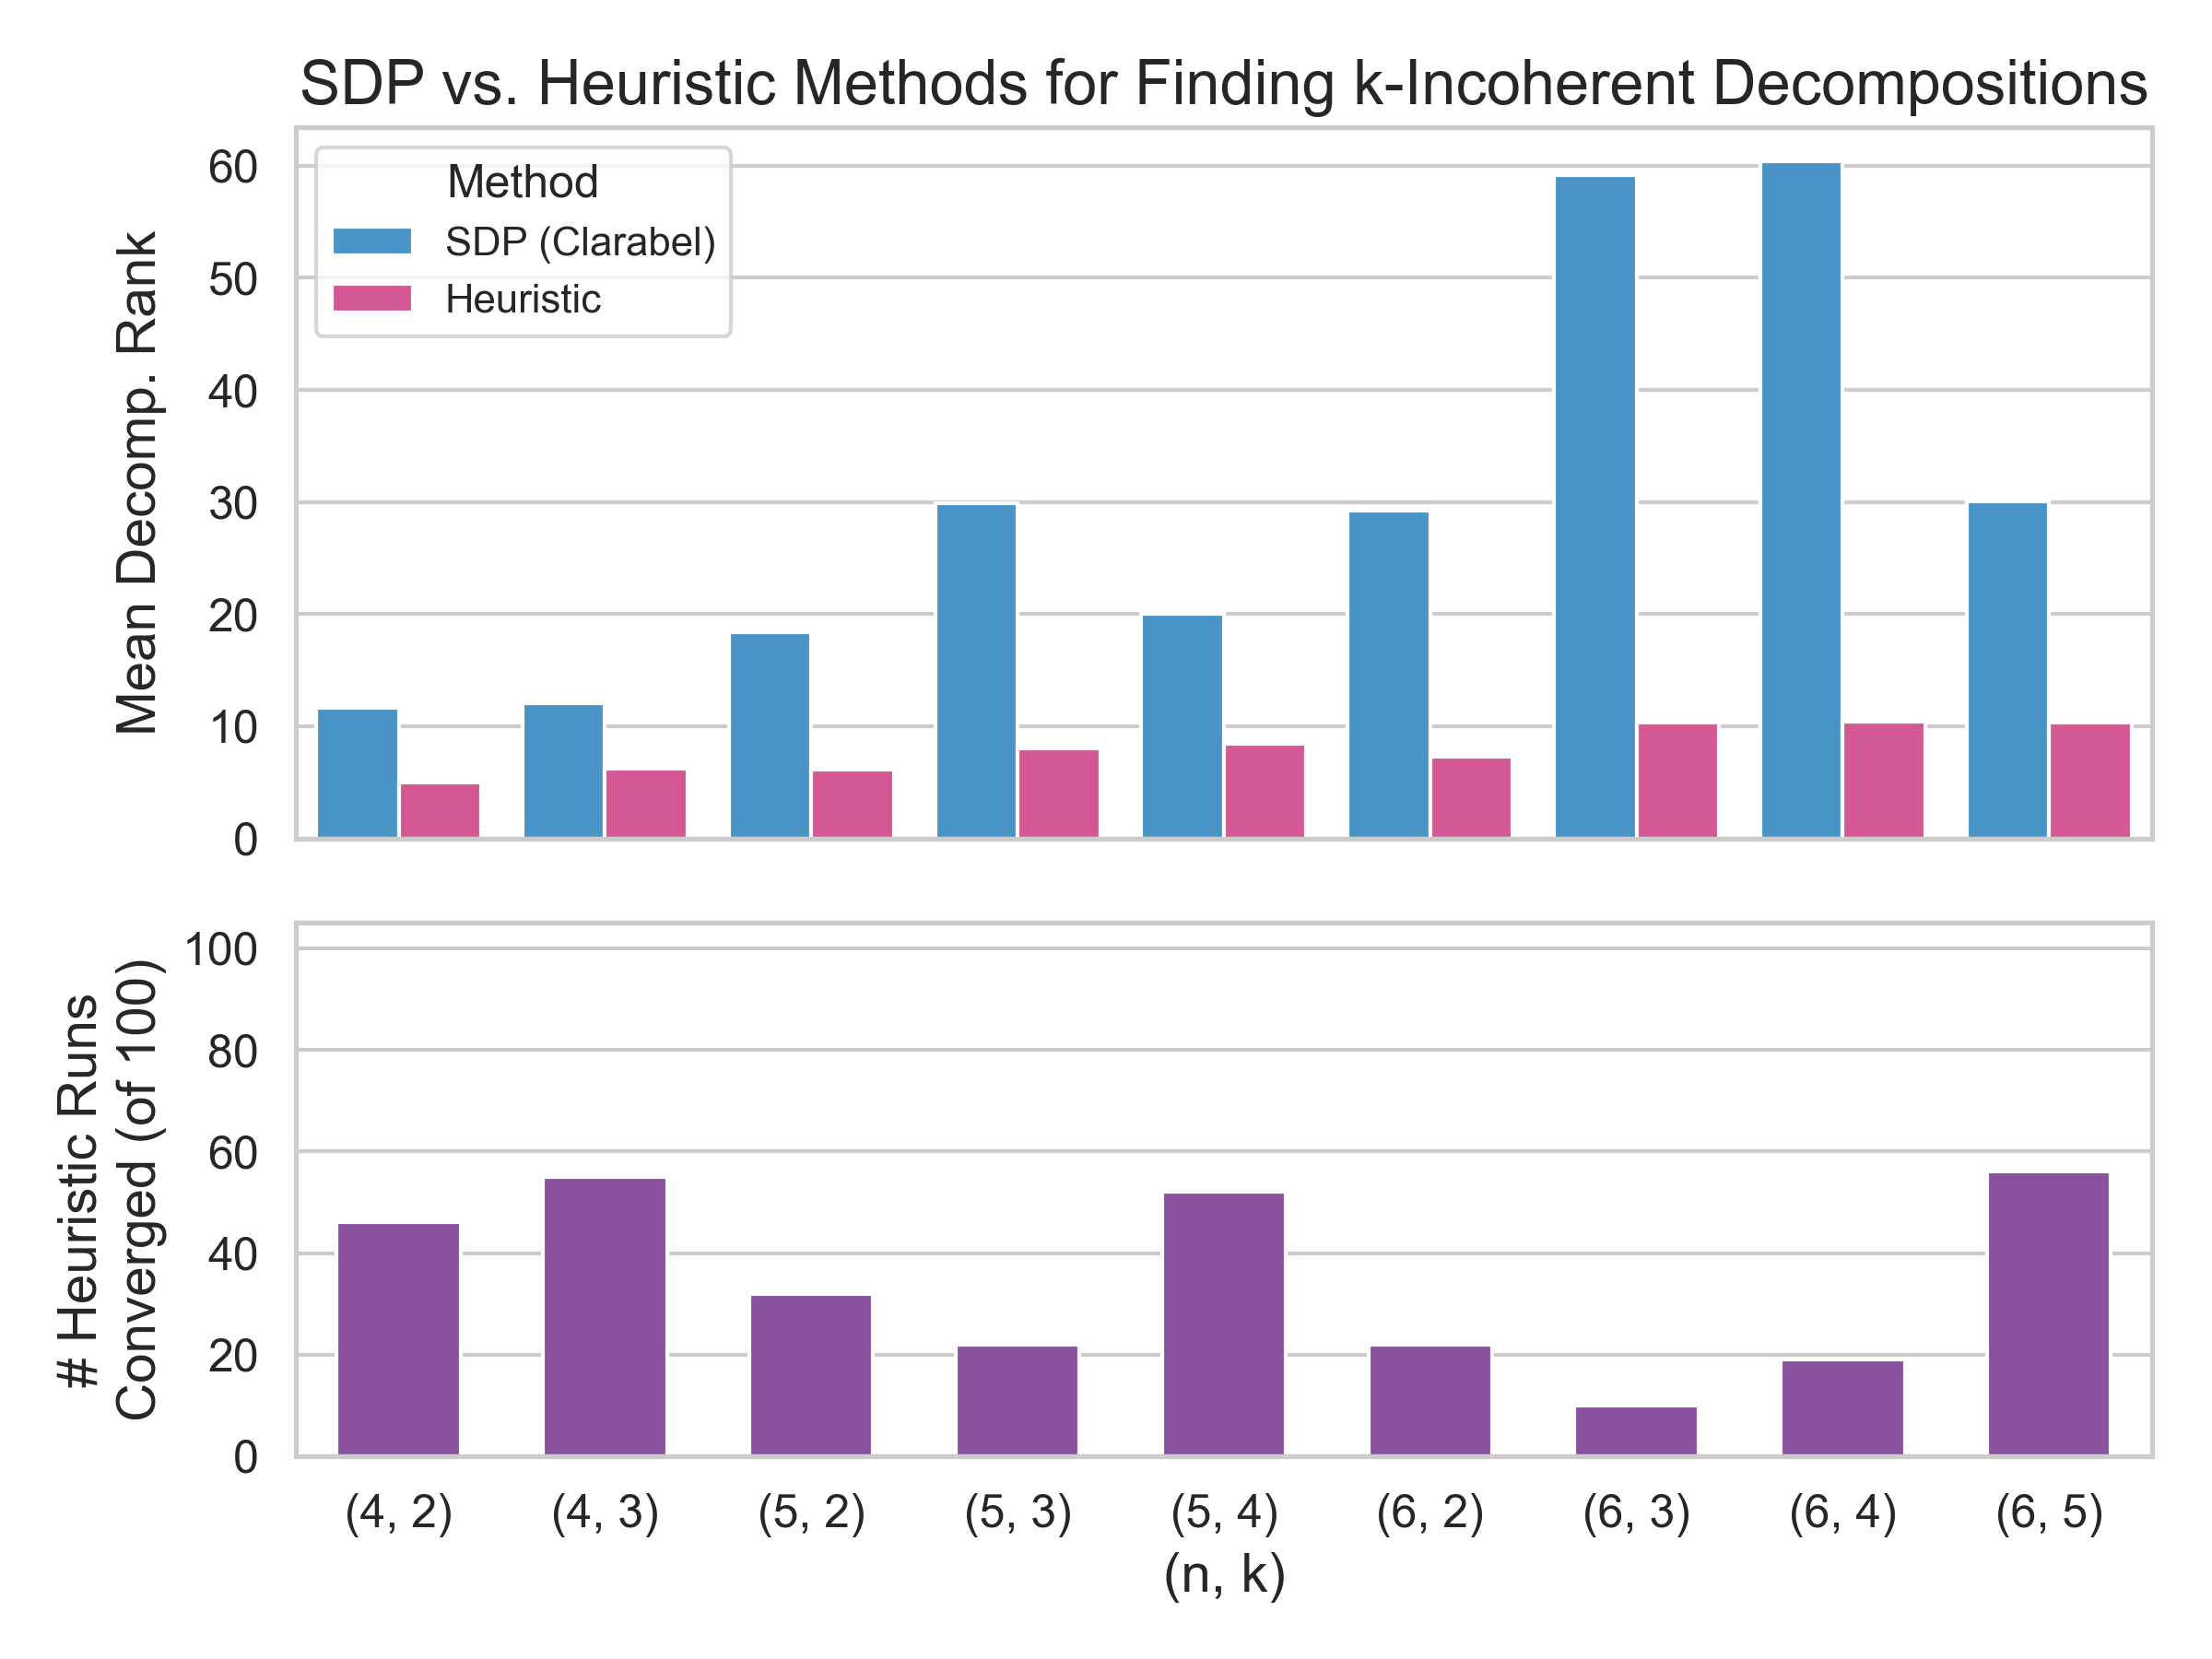
\includegraphics[height=6.1cm]{assets/sdp_vs_heuristic.png}}
        \vspace*{-0.3cm}
        \caption{The maximum-eigenvalue heuristic with cyclic coordinate descent converges \emph{$\mathbf{\approx\!35\%}$} of the time to within Frobenius distance $< 10^{-14}$, requiring only \emph{$\mathbf{\approx\!32.3\%}$} as many terms as SDP when successful.}
        \label{fig:sdp-vs-heuristic}
    \end{figure}
}

\section{Conclusion}

\subsection{Thank you for listening!}

\frame{
    \frametitle{Thank you for listening!}
    \begin{figure}
        \centering
        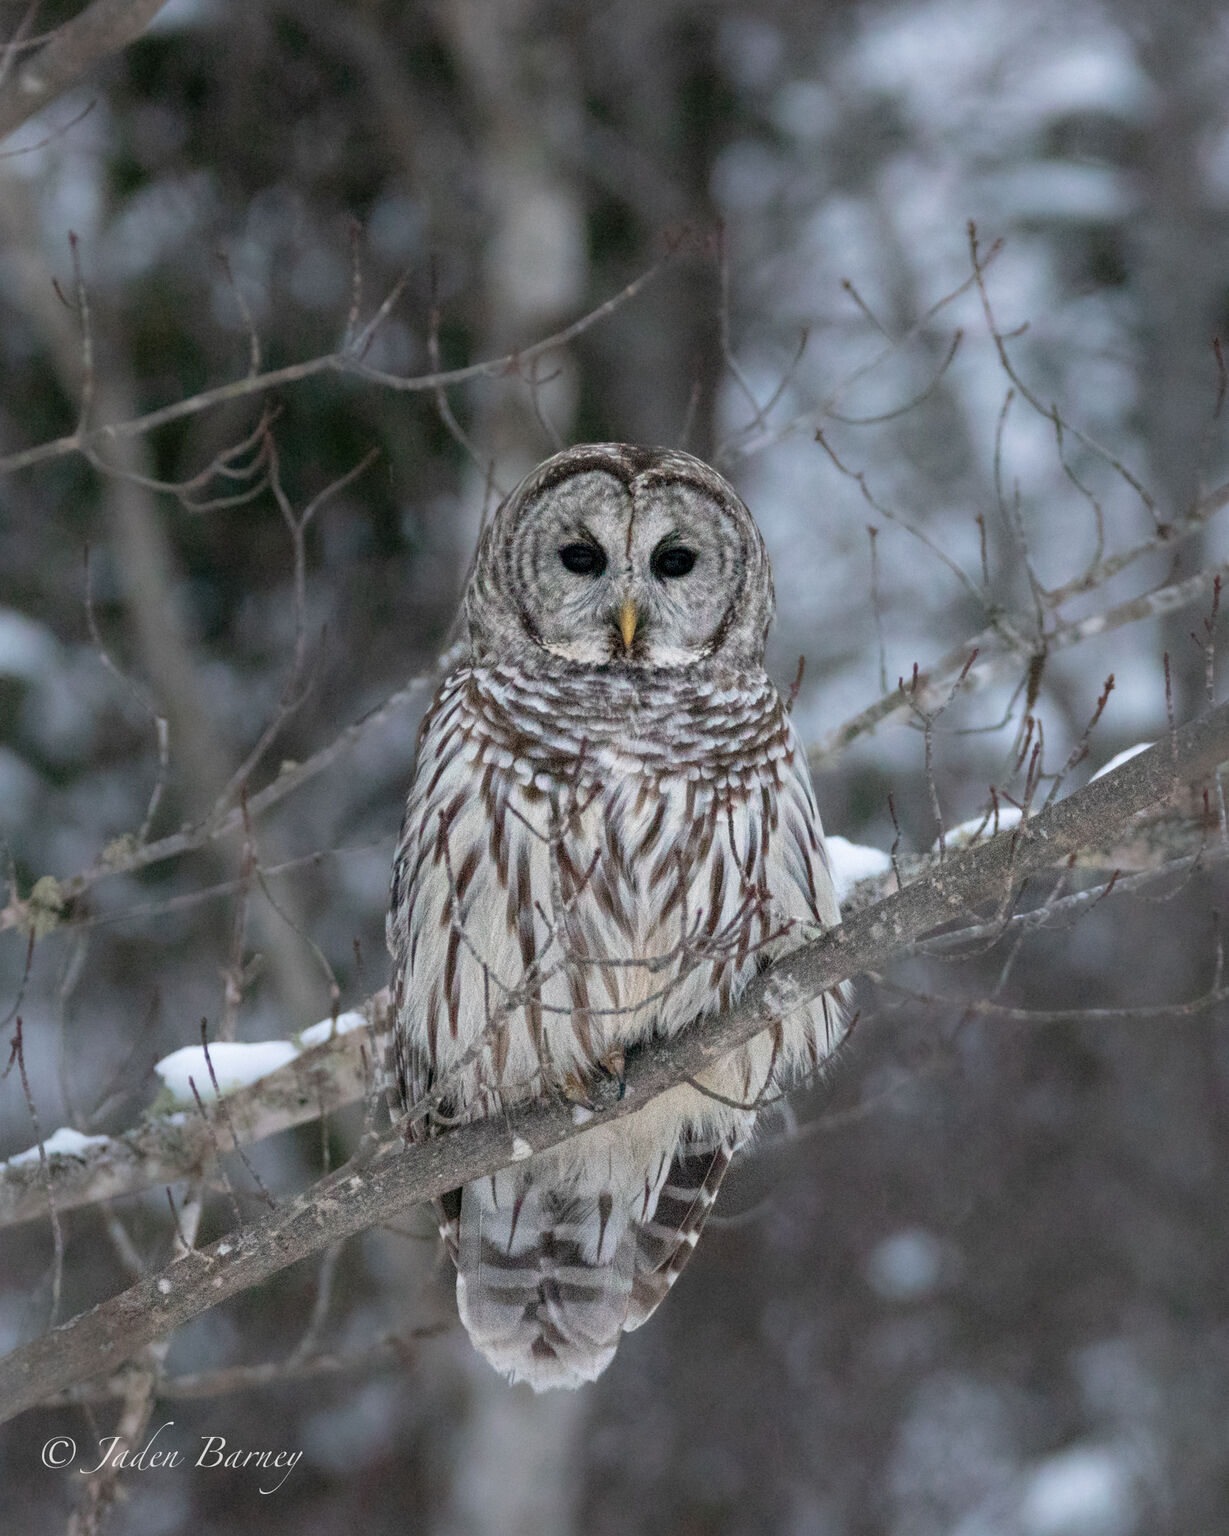
\includegraphics[height=6.1cm]{assets/owl_midgic_jaden_comp.jpg}
        \vspace*{-0.3cm}
        \caption{A \emph{barred owl} in Midgic, NB---approximately two hours away from Charlottetown, PE when travelling at the maximum air-speed velocity of an unladen owl. [Credit: \emph{Jaden Barney}.]}
        \label{fig:owl-midgic}
    \end{figure}
}

\end{document}
